\documentclass[conference]{IEEEtran}
\IEEEoverridecommandlockouts
\usepackage{cite}
\usepackage{amsmath,amssymb,amsfonts}
\usepackage{algorithmic}
\usepackage{graphicx}
\usepackage{textcomp}
\usepackage{xcolor}
\def\BibTeX{{\rm B\kern-.05em{\sc i\kern-.025em b}\kern-.08em
    T\kern-.1667em\lower.7ex\hbox{E}\kern-.125emX}}
\begin{document}

\title{Use of SSH Certificates to Reduce Risk in Large Distributed Computing Environments\\
}

\author{\IEEEauthorblockN {Austin Krauza}
\IEEEauthorblockA{\textit{Tandon School of Engineering at New York University}\\
New York, United States \\
ak4769@nyu.edu}}

\maketitle

\begin{abstract}
With the movement away from passwords towards more cryptographically secure methods, SSH public/private key pairs have become more prevalent amongst technologists to access remote systems. When hardening a new Linux or Unix server, one of the first tasks of the administrator should be to disable password authentication, thereby reducing the attack vector brute forcing logins against the system. However, while the use of SSH keys over password authentication reduces the effectiveness of brute force attacks, by itself it is still only "one factor authentication"; it replaces something you know (password) for something you have (the keypair). Additionally, just as with a password, there is the same risk of the keypair being leaked or stolen. With the usage of a signed SSH Certificate, a known and trusted source (i.e., a Certificate Authority) can cryptographically "sign" and scope a SSH key, restricting access a specific environment as a pre-determined user for a short period of time. This paper will identify how the use of a SSH Certificates increases the auditability of users in a shared/multi-tenant environment, reduces the footholds for lateral movement by a bad actor, and decreases the blast radius when a key pair is leaked.
\end{abstract}
\begin{IEEEkeywords}
ssh, rsa, secure shell, distributed computing, risk, security, certificates
\end{IEEEkeywords}

\section{Introduction}
SSH (Secure Shell) key pairs are one of the most secure ways to authenticate to a system when using the SSH protocol. When accessing a system, traditionally users would authenticate using a username and password combination, which only provides one factor authentication (something you know). If a user’s credentials were obtained and used by a bad actor (through a phishing attempt, credential dump, password crack, etc.), that threat actor would be able to trivially impersonate the original user with their full un-scoped entitlements. Additionally, just like passwords, users often reuse the same SSH key pair between multiple services and systems \cite{yolen}, therefore creating a single point of compromise and an increased security boundary should that credential fall out of control of the user. As mentioned by Ylonen who studied various financial intuition's usage of SSH keys, "...many of the companies ... had several million keys authorized to log in across tens of thousands, sometimes over a hundred thousand servers. In some cases a single key can access thousands of servers." \cite{yolen}.

In terms of managing SSH keys from an infrastructure point of view, a user’s public portion of the key pair must be installed into each system which that user needs to access (typically by the user themselves). This method creates a circular dependency on the use of passwords to install the public key before password-less authentication (or password/key pair combination) can be used. Furthermore, this management style does not scale in large distributed systems wherein an entity might need to access any one several hundred hosts at any point (think a Kubernetes cluster) or the public key pair list could be removed when the system undergoes regular hygiene and the file system is cleared. 

\begin{figure}
\centerline{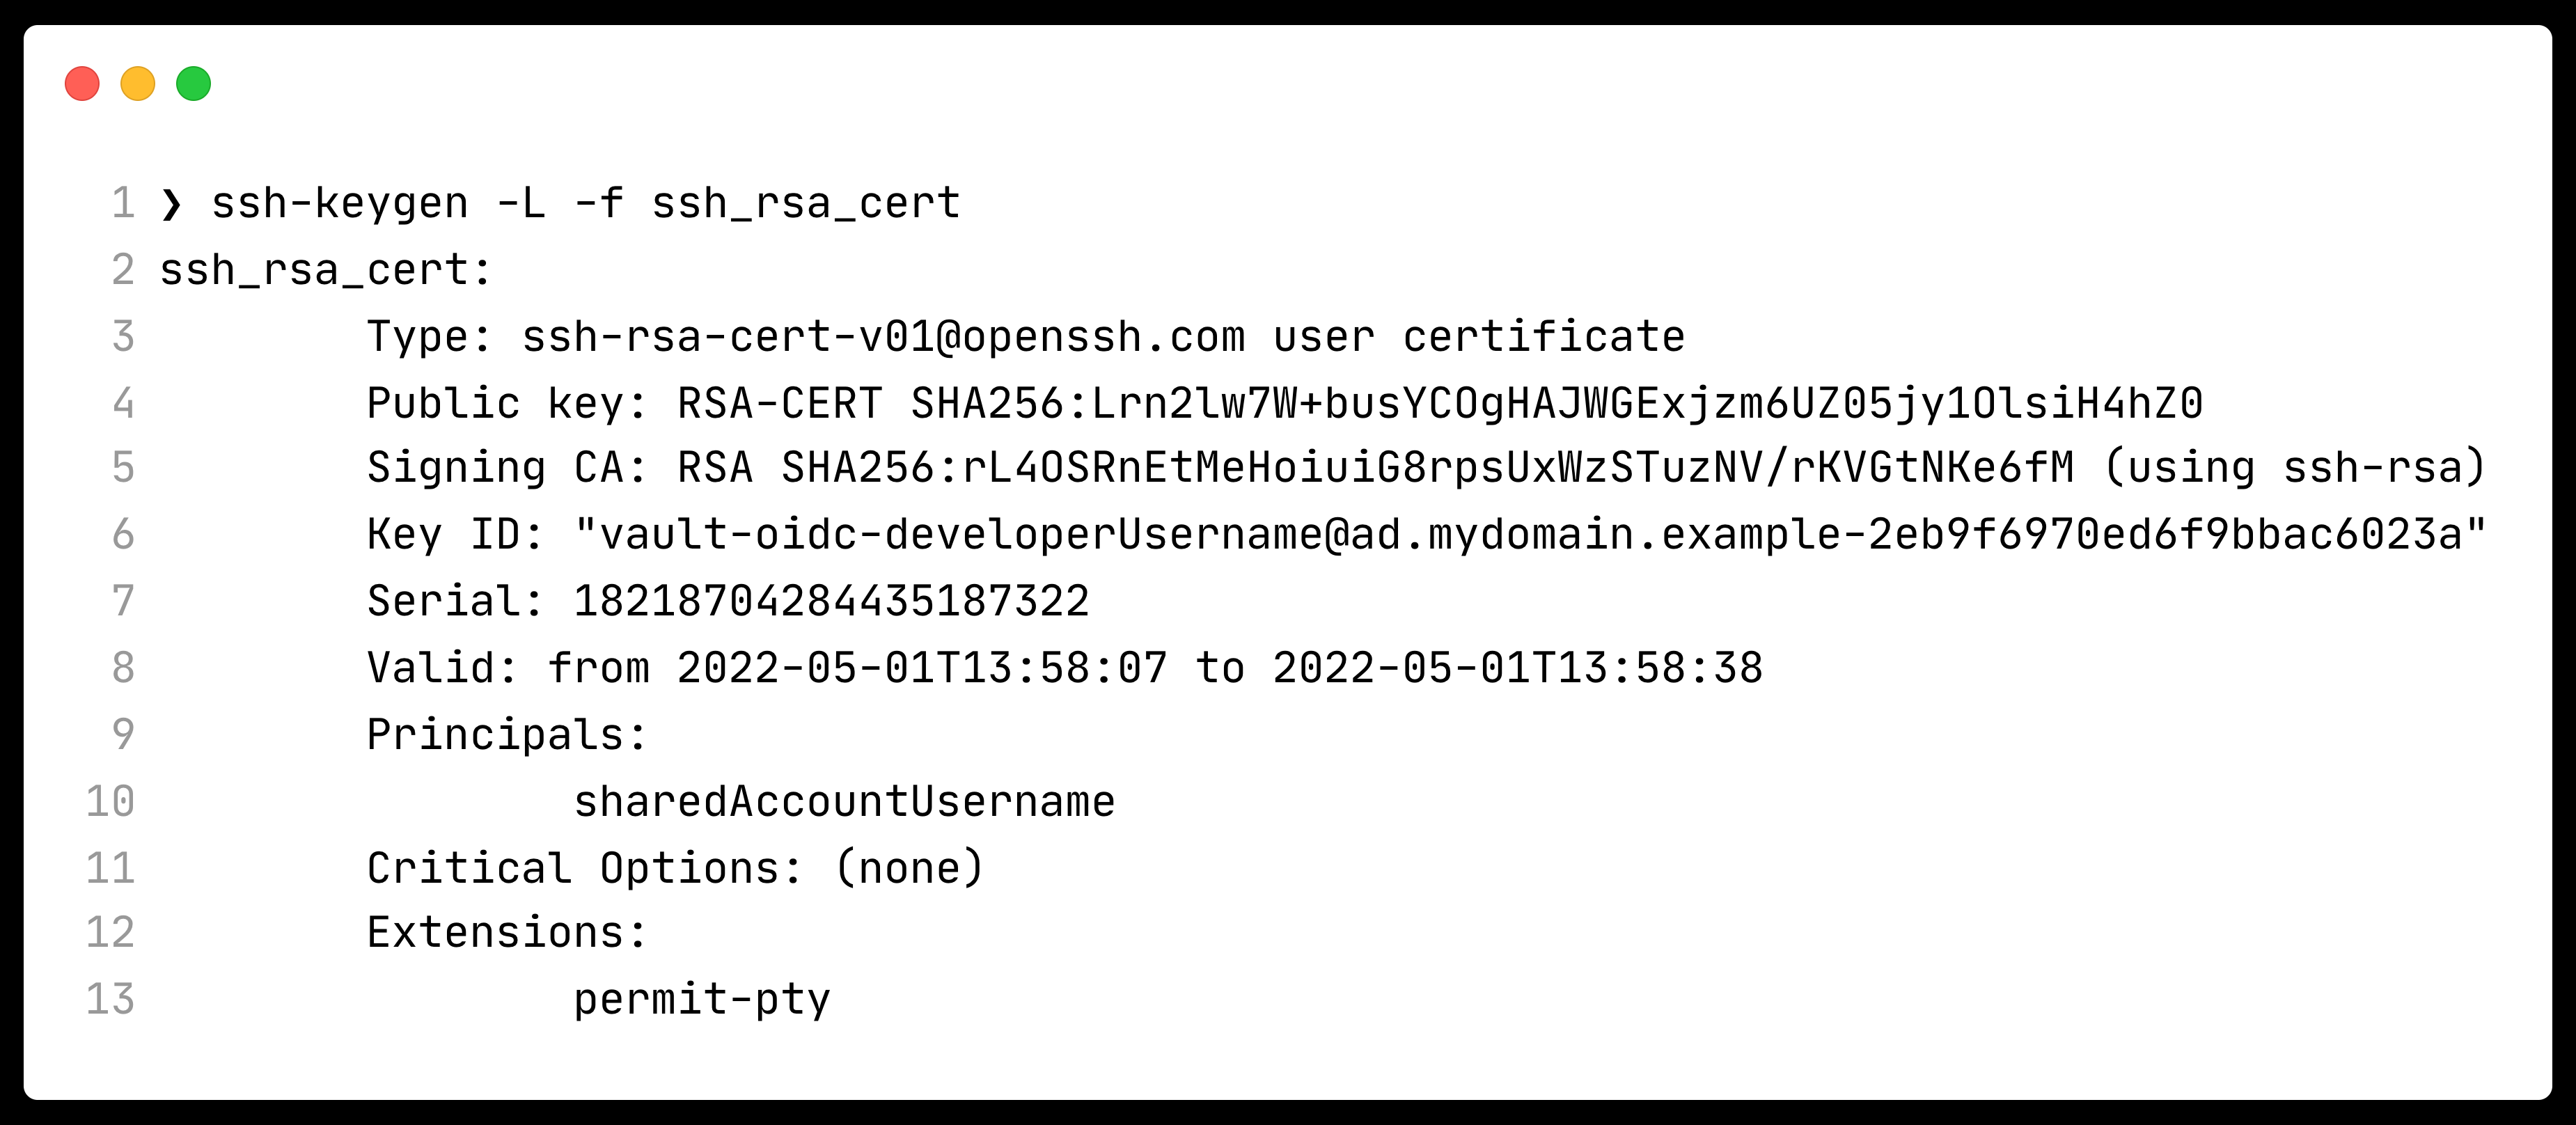
\includegraphics[width=\columnwidth,keepaspectratio]{keypair.png}}
\caption{Contents of a Signed SSH Certificate}
\label{fig:Keypair}
\end{figure}

\section{Hypothesis}
The author of this paper proposes the broader adoption of SSH Certificates as an alternative/addition to password-based authentication and/or the use of a traditional SSH key pair. By using a SSH Certificate, an entity wanting to access a system would first declare their intent along with a public key to an authoritative system to be signed. This system would then verify the provided information and cryptographically issue a short lived (and scoped) certificate to the user.

The contents of a sample SSH Certificate is shown in Figure \ref{fig:Keypair}, including important fields such as the \textit{Key ID}, \textit{Valid} period, \textit{Principals} (i.e., the user which the certificate can be used to authenticate as), and the allowed \textit{Extensions}. For those familiar with a JSON Web Token (JWT), this format should be quite analogous. The use of a SSH Certificate signed by a trusted Certificate Authority accomplishes three main points: first, it dramatically decreases the management overhead needed to manage individual user’s SSH public keys on hosts, next it increases audit capabilities by creating an independent and immutable system recording the “signing” of a key pair to access a particular system, and finally it decreases the security boundary should a user’s private key be compromised by a bad actor.

As discussed earlier, SSH key pairs are extremely vulnerable to leakage and are traditionally high touch in terms of management across large scale distributed environments. For example, if a user is part of an application development team which needs to access six or seven different hosts (across different data centers, environments, etc.), that user’s SSH public key must be added to each different server either manually or by some other automation pipeline. Additionally, if the user no longer needs access, the administrator of the host must delete and remove that user’s key from the host. Traditionally, a first-time user would login with a keyboard authentication method, and then subsequently add their public key to the \textit{authorized{\_}keys} file in their home directory. With the proposed broader adoption of Signed SSH Certificates, authorization for accessing the system is now externalized to a third-party (e.g., Active Directory, Okta, Keycloak, etc.) where permissions can easily be added or dropped (and audited) as the role of the user changes.

\begin{table}[ht]
\caption{Threat Model for Public/Private Key Pairs}
\resizebox{\columnwidth}{!}{
\label{table:ThreatModel}
\begin{tabular}{p{0.2\linewidth} p{0.2\linewidth} p{0.6\linewidth}}
\multicolumn{1}{c}{Threat} &
\multicolumn{1}{c}{Desired Property} & 
\multicolumn{1}{c}{Issue} \\
\hline
Spoofing & Authenticity & There is no guarantee that the entity using the SSH keypair is the actual true owner of the SSH key. In some environments, the same SSH key is shared amongst teams or individuals (e.g., in the case of AWS EC2 instances where one key-pair is assigned). \\ \hline
Tampering & Integrity & If an entity’s SSH key is compromised in any way, that public key must be removed from every server and resource to which it has been added (e.g., authorized{\_}keys). This is a very intensive process and requires that strict inventory be kept of everywhere the key is used. \\ \hline
Repudiation & Non-repudiability & SSH key pairs are by nature uncontrolled. Being that key pairs are not "vended" or managed/issued by an outside system (they are typically generated by users and added to the authorized{\_}keys file), there is no guarantee that an "authorized keypair" is genuinely authorized to have access to the system or resource. \\ \hline
Information disclosure & Confidentiality & SSH keys can be leaked by code deploy pipelines or human error (e.g., committing to SCM). Being that there is no time-to-live (TTL) on an SSH keypair, and a lack of any other viable revocation method, there is limited traceability and inherent revocation process in the event of a leak. \\ \hline
Elevation of Privilege & Authorization & Generally, SSH key pairs (using the \textit{authorized{\_}keys} file on *nix hosts) need to be added to the initial user which an entity is using to log into the box. A user can then use the sudo or su command to switch users, provided they are of the appropriate administrative group. However, this introduces group management and audit issues when a user needs to "become" or authenticate as another user.
\end{tabular}
}
\end{table}

The threat model as described in Table \ref{table:ThreatModel} identifies a variety of different attack scenarios for accessing a system using traditional SSH key pairs. The model used for this paper was the \textit{STRIDE} model, which is a model developed by Microsoft to realize the absence of desired security properties of a system or process. The key threats of SSH key pairs recognized by this paper are spoofing, repudiation, information disclosure, and elevation of privilege. The threats of spoofing, repudiation, and information disclosure are related to the trust and "lack of control" of a user's key pair. Just because a public key is present on a host in the \textit{authorized{\_}keys} file, there is no guarantee that the key is "in control" by the user and has not been leaked or compromised. In terms of persistence, if a "bad" actor were able to compromise a host and inject their \textit{own} public key into {authorized{\_}keys}, the "bad" actor could potentially maintain access even if the "good" user used a new keypair.

\section{Motivating Example}

In the proposed example flow described in Figure \ref{fig:SignedKeyFlow}, we assume the organization leverages Active Directory as their directory manager of choice, and the user has been added to the appropriate entitlement groups within the directory. When the user needs to access a protected resource (e.g., a database server), they will first authenticate to the identity provider (using either OAuth2 or SAML) which authenticates and later authorizes the user based on their roles within the directory, producing a JSON Web Token (JWT) with their roles and claims. The user will then use the JWT to authenticate to an application which has access to a trusted Certificate Authority's private key. The purpose of this application is to verify the intent of the user, and eventually issue a signed certificate certifying the time to live and conditions of authentication. Upon a successful signing, the user is returned a signed certificate from the application, which they will then use as part of the authentication process to the SSH protected resource.

Besides certificates, the typical solution to "securing" SSH key pairs is the use a passphrase to encrypt the key pair. While the use of a passphrase solves for the spoofing and/or integrity, it does not address repudiation. When a public key is added into the \textit{authorized{\_}keys} file, there is no guarantee that the key(s) contained within that file are that of the user and not of a bad actor. This is because key pairs are typically generated by a user in their own environment and not generated by a trusted or auditable source. With the use of a SSH certificate and signing, a user could theoretically generate a new public and private key pair each and every time they connect to a system and it would not matter. In this case, the system/host is only checking that the key pair is accompanied by a certificate signed by a trusted authority (CA) and that the hash of the provided key pair matches contained in the certificate (as shown in Figure \ref{fig:Keypair}). There is no prior knowledge of the keypair's public key pre-authentication.

\begin{figure}
\centerline{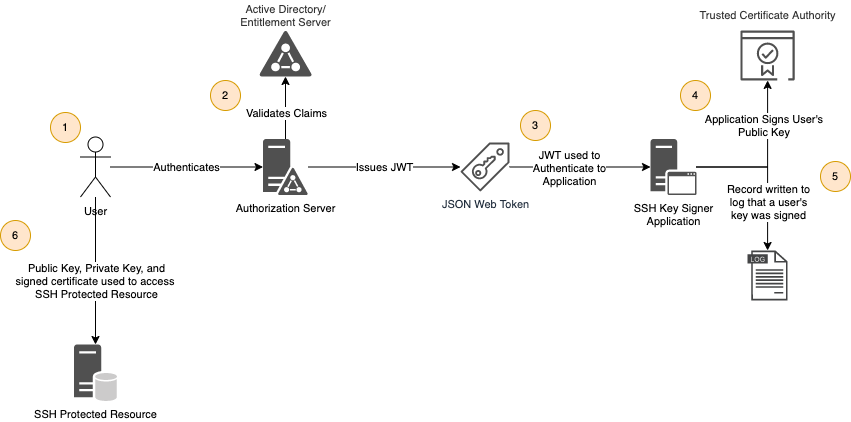
\includegraphics[width=\columnwidth,keepaspectratio]{SignedKeysFlow.png}}
\caption{Proposed solution for generating a SSH Certificate for a User}
\label{fig:SignedKeyFlow}
\end{figure}

\begin{table}[ht]
\caption{Comparison of Developer Experience \& Time using Signed SSH Certificates as compared to Public/Private Key Pairs}
\resizebox{\columnwidth}{!}{
\label{table:TimeComparisonDeveloper}
\begin{tabular}{p{0.4\linewidth} p{0.3\linewidth} p{0.3\linewidth}}
\multicolumn{1}{c}{Action} &
\multicolumn{1}{c}{Public/Private Key Pair} & 
\multicolumn{1}{c}{SSH Certificate} \\
\hline
Install/Rotation of SSH public key onto 10 hosts & 4 minutes * 10 hosts = 40 minutes & N/A (as CA is installed as part of infrastructure build process) \\ \hline
Initiating an SSH session into a host & 15 seconds & 60 seconds (assuming SSO of user to “Key Signing” Application) \\ \hline
\end{tabular}
}
\end{table}

\begin{table}[ht]
\caption{Comparison of Time Spent Maintaining Signed SSH Certificates as compared to Public/Private Key pairs}
\resizebox{\columnwidth}{!}{
\label{table:TimeComparisonMaintenance}
\begin{tabular}{p{0.4\linewidth} p{0.3\linewidth} p{0.3\linewidth}}
\multicolumn{1}{c}{Action} &
\multicolumn{1}{c}{Public/Private Keypair} & 
\multicolumn{1}{c}{SSH Certificate} \\
\hline
Install CA onto 10 hosts & N/A & \begin{tabular}[c]{@{}l@{}}2 minutes per host \\ or\\ 15 seconds with \\ automation\end{tabular} \\ \hline
Management of Certificate Authority (CA) & N/A & 3 hours every 2 years \\ \hline
Maintenance of “Key Signing” Application & N/A & 40 hours per year \\ \hline
Identification of unauthorized SSH key pair usage post key compromise & 24 hours & N/A \\ \hline
Removal of SSH key from environment after employee separation & 2 hours & N/A \\ \hline
Auditing of SSH keypair usage & 8 hours per month & 15 minutes \\ \hline
\end{tabular}
}
\end{table}

\section{Evidence}

The data used for this experiment and analysis is purely anecdotal based on the experiences of the author as an engineer in the Distributed Computing and Cloud space. As with the best of security controls (and the use of Signed SSH Certificates certainly falls into this category), care must be taken to ensure that the control itself does not start to become a burden or hindrance on the user (e.g., the developer). Once the control begins to impede on productivity or ease of accessibility for the user, the user will stop following the control and start to find workarounds to avoid the complicated process. Table \ref{table:TimeComparisonDeveloper} speaks to some of this hindrance. Using a standard SSH key pair could be seen by users by allowing them to connect to a host "passwordless" in as little as fifteen seconds, while as it taking upwards of 60 seconds with the use of Signed Certificates. The added time is due to the user having to authenticate to the issuing system, provide details of the host they want to connect to, and then wait for the system to generate and sign the certificate. Some users could see this increase in time as a barrier to their productivity, when rather it should be seen as a way to decrease risk to the host and environment.

In terms of administrative overhead and maintenance, there is additional work that must be taken on by the Systems Administration (SA) and Cybersecurity (Cyber) teams to keep the system operational. With the use of Public/Private keypairs, there is little to no involvement by either the SA or Cyber teams when adding a new keypair for a user to a system. However, with the use of Signed Certificates, there is the assumption that there is a Certificate Authority (CA), a Single Sign On (SSO) or Identity Provider (IDP) to authenticate a user is present, along with an entitlement management system, and finally a vaulting or other vault like application which is able to parse and verify the input from a user and conditionally issue a signed Certificate. While most of these systems are already in use by an organization, they might not be -- requiring additional time and effort being spent on maintaining the system, as shown in Table \ref{table:TimeComparisonMaintenance}. 

\section{Related Work}
Several researchers have studied various organization's use of Public Key Infrastructure (PKI), and how it could be applied to either SSH logins or One Time Passwords (OTP). In "A Design of One-Time Password Mechanism Using Public Key Infrastructure", H. Kim, et. al. discusses various proposals for implementing a secure authentication system using PKI \cite{kim}. Of the solutions introduced, the "Certificate Issuance and Registration" methodology is most similar and provides precedence for the solution set forth in this paper. In the "Certificate Issuance and Registration" scenario, a user would contact a Registration Authority (RA) which would then transfer to a Certificate Authority the request and user information \cite{kim}. After being validated, a reference number and approval would be returned back to the user, and that reference would be used to issue a certificate. While this does not completely match the solution proposed, it does provide a basis for validating a user's identity and intent before allowing the issuance of a certificate by a Certificate Authority.

\section{Summary}
Based on the above solution set forth by the author, additional layers of security are put in place to avoid the abuse and misuse of SSH key pairs in a distributed key environment. Through the use of a Certificate Authority (CA) as a trusted and official source of truth, you can validate that the user accessing the system is the intended entity, and with both time and permissions scoped. While the level of effort is higher to maintain such Certificate and Registration Authorities, there is increased control and repudiation within the system.

\begin{thebibliography}{00}
\bibitem{kim} H. Kim, H. Lee, K. Lee and M. Jun, "A Design of One-Time Password Mechanism Using Public Key Infrastructure," 2008 Fourth International Conference on Networked Computing and Advanced Information Management, 2008, pp. 18-24, doi: 10.1109/NCM.2008.77.
\bibitem{kumagai} M. Kumagai, Y. Musashi, D. A. L. Romana, K. Takemori, S. Kubota and K. Sugitani, "SSH Dictionary Attack and DNS Reverse Resolution Traffic in Campus Network," 2010 Third International Conference on Intelligent Networks and Intelligent Systems, 2010, pp. 645-648, doi: 10.1109/ICINIS.2010.9.
\bibitem{yolen} T. Ylonen, "SSH Key Management Challenges and Requirements," 2019 10th IFIP International Conference on New Technologies, Mobility and Security (NTMS), 2019, pp. 1-5, doi: 10.1109/NTMS.2019.8763773.
\bibitem{zheng} L. Zheng, C. Zhao and Z. Wang, "The SSH Protocol Audit System Based on Proxy Technology," 2013 International Conference on Computational and Information Sciences, 2013, pp. 1489-1492, doi: 10.1109/ICCIS.2013.392.

\end{thebibliography}

\end{document}